%%%%%%%%%%%%%%%%%%%%%%%%%%%%%%%%%%%%%%%%%%%%%%%%%%%%%%%%%%%%%%%%%%%%%%%%%%%%%%%%%%%%%%%
%%%%%%%%%%%%%%%%%%%%%%%%%%%%%%%%%%%%%%%%%%%%%%%%%%%%%%%%%%%%%%%%%%%%%%%%%%%%%%%%%%%%%%%
% 
% This top part of the document is called the 'preamble'.  Modify it with caution!
%
% The real document starts below where it says 'The main document starts here'.


\documentclass[12pt]{article}

\usepackage{amssymb,amsmath,amsthm}
\usepackage[top=1in, bottom=1in, left=1.25in, right=1.25in]{geometry}
\usepackage{fancyhdr}
\usepackage{listings}
\usepackage{enumerate}
\usepackage{hieroglf}
\usepackage{oands}
\usepackage{arevmath}
\usepackage{relsize}
\usepackage{times,txfonts}
\usepackage{graphicx}
\usepackage{float}

\newtheoremstyle{homework}% name of the style to be used
  {18pt}% measure of space to leave above the theorem. E.g.: 3pt
  {12pt}% measure of space to leave below the theorem. E.g.: 3pt
  {}% name of font to use in the body of the theorem
  {}% measure of space to indent
  {\bfseries}% name of head font
  {:}% punctuation between head and body
  {2ex}% space after theorem head; " " = normal interword space
  {}% Manually specify head
\theoremstyle{homework} 

% Set up an Exercise environment and a Solution label.
\newtheorem*{exercisecore}{Exercise \@currentlabel}
\newenvironment{exercise}[1]
{\def\@currentlabel{#1}\exercisecore}
{\endexercisecore}

\newcommand{\localhead}[1]{\par\smallskip\noindent\textbf{#1}\nobreak\\}%
\newcommand\solution{\localhead{Solution:}}

%%%%%%%%%%%%%%%%%%%%%%%%%%%%%%%%%%%%%%%%%%%%%%%%%%%%%%%%%%%%%%%%%%%%%%%%
%
% Stuff for getting the name/document date/title across the header
\makeatletter
\RequirePackage{fancyhdr}
\pagestyle{fancy}
\fancyfoot[C]{\ifnum \value{page} > 1\relax\thepage\fi}
\fancyhead[L]{\ifx\@doclabel\@empty\else\@doclabel\fi}
\fancyhead[C]{\ifx\@docdate\@empty\else\@docdate\fi}
\fancyhead[R]{\ifx\@docauthor\@empty\else\@docauthor\fi}
\headheight 15pt

\def\doclabel#1{\gdef\@doclabel{#1}}
\doclabel{Use {\tt\textbackslash doclabel\{MY LABEL\}}.}
\def\docdate#1{\gdef\@docdate{#1}}
\docdate{Use {\tt\textbackslash docdate\{MY DATE\}}.}
\def\docauthor#1{\gdef\@docauthor{#1}}
\docauthor{Use {\tt\textbackslash docauthor\{MY NAME\}}.}
\makeatother

% Shortcuts for blackboard bold number sets (reals, integers, etc.)
\newcommand{\Reals}{\ensuremath{\mathbb R}}
\newcommand{\Nats}{\ensuremath{\mathbb N}}
\newcommand{\Ints}{\ensuremath{\mathbb Z}}
\newcommand{\Rats}{\ensuremath{\mathbb Q}}
\newcommand{\Cplx}{\ensuremath{\mathbb C}}
%% Some equivalents that some people may prefer.
\let\RR\Reals
\let\NN\Nats
\let\II\Ints
\let\CC\Cplx

%%%%%%%%%%%%%%%%%%%%%%%%%%%%%%%%%%%%%%%%%%%%%%%%%%%%%%%%%%%%%%%%%%%%%%%%%%%%%%%%%%%%%%%
%%%%%%%%%%%%%%%%%%%%%%%%%%%%%%%%%%%%%%%%%%%%%%%%%%%%%%%%%%%%%%%%%%%%%%%%%%%%%%%%%%%%%%%
% 
% The main document start here.

% The following commands set up the material that appears in the header.
\doclabel{Math 316: HW 4}
\docauthor{Stefano Fochesatto}
\docdate{\today}

\begin{document}


\textbf{Section 4.3}
\begin{exercise}{6} Prove that 7 is the only prime of the form [Hint factor $n^3 - 1$ into $(n-1)(n^2+n+1)$.], 
  \begin{equation*}
    n^3 - 1
  \end{equation*}
  
  \solution Considering the hint let's factor $n^3 - 1$ into $(n-1)(n^2+n+1)$. Now let $z$ be a prime number and
  suppose that, 
  \begin{equation*}
    z = (n-1)(n^2+n+1).
  \end{equation*}
  Since $z$ is prime by the fundamental theorem of arithmetic we know that either $(n-1) = 1$ or $(n^2+n+1) = 1$. 
  Suppose that $(n^2+n+1) = 1$, through some algebra we can see that, 
  \begin{align*}
    (n^2+n+1) &= 1,\\
    n^2+n &=0,\\
  n(n+1)&=0.
  \end{align*}
  Therefore we have that $n = 0,-1$ however substituting back into our original equation we get, 
  \begin{equation*}
    (0)^3 - 1 = -1
  \end{equation*}
  \begin{equation*}
    (-1)^3 - 1 = -2
  \end{equation*}
  and neither solution is prime therefore it must be the case that $(n-1) = 1$ which gives us $n = 2$. Substituting
  $n = 2$ we get,
  \begin{equation*}
    (2)^3 -1 = 7.
  \end{equation*}
  Thus 7 is the only prime of the form $n^3 - 1$. 
\end{exercise}
\vspace{.5in}






\begin{exercise}{7} Find a set of four consecutive odd integers of which three are primes, 
  and a set of five consecutive odd integers of which four are prime.\\
  \solution For the set of four consecutive odd integers consider the set, 
  \begin{equation*}
    3,5,7,9.
  \end{equation*}
  Note that $3,5,7$ are prime, and $9$ is not since $9 = 3^2$. For the set of five consecutive odd numbers 
  consider,
  \begin{equation*}
    3,5,7,9,11.
  \end{equation*} 
  Note that $11$ is prime, so there are now four prime numbers. 
\end{exercise}
\vspace{.5in}


\begin{exercise}{15} Find the $gcd(272,1479)$.\\
  \solution We will proceed by using the Euclidean algorithm, 
  \begin{align*}
    1479 &= (5)*272 + 119,\\
    272 &= (2)*119 + 34,\\
    119 &= (3)*34 + 17,\\
    34 &= (2)*17 + 0.
  \end{align*}
  Therefore we get that $gcd(272,1479) = 17$.
\end{exercise}
\vspace{.5in}






\begin{exercise}{16b} Use the Euclidean algorithm to find $x$ and $y$ such that, 
  \begin{equation*}
    gcd(24,138) = 24x + 138y. 
  \end{equation*}

  \solution First we must use the Euclidean algorithm to find $gcd(24,138)$,
\begin{align*}
  138 &= (5)24 + 18,\\
  24 &= (1)18 + 6,\\
  18 &= (3)6 + 0.
\end{align*}
Therefore we have that $gcd(24,138) = 6$. To solve for $x$ and $y$ we use the Euclidean algorithm
backwards, 
\begin{align*}
  6 &= 24 - 18,\\
  6 &= 24 - (138 - (5)24),\\
  6 &= 24 - 138 + (5)24,\\
  6 &= (6)24 + (-1)138.\\
\end{align*}
Therefore we have that $x = 6$ and $y = -1$.

\end{exercise}
\vspace{.5in}




\textbf{Section 4.4}
\begin{exercise}{4b}
\end{exercise} From Ptolemy's value $chord(1) = 1;2,50$ and using an inscribed 360-gon to approximate 
the circumference of a circle, obtain his approximation of $\pi$.\\
\solution We know that the $\pi$ is the ratio between a circle's circumference and diameter. Using Ptolemy's
value for a the length of a 1 degree chord, we can find an approximation for the circumference using the perimeter of an inscribed 
360-gon. Note that eac side of an inscribed 360-gon will have the length $chord(1) = 1;2,50$ so we know that,
\begin{equation*}
  C \approx 360 * 1;2,50 = 6,0; * 1;2,50
\end{equation*}
Dividing by a diameter of $2,0;$ we get that, 
\begin{align*}
 \pi &\approx \frac{6,0;}{2,0;} * 1;2,50\\
 &= 3; * 1;2,50\\
   &= 3;6;150 \\
   &\approx 3.14166
\end{align*}
\vspace{.5in}




\textbf{Section 4.5}

\begin{exercise}{10} Given a spiral, place the angle to be trisected so that the vertex 
  and the initial side of the angle coincide with the initial point of the spiral and the
   initial position $OA$ of the rotating ray. Let the terminal side of the angle intersect the
    spiral of $P$. Trisect the segment $OP$ at the points $Q$ and $R$, and draw circles with center at 
    $O$ and with $OQ$ and $OR$ as radii. Prove that if these circles meet the spiral in points $U$ and $V$ , 
    then the lines $OU$ and $OV$ will trisect $\angle AOP$.\\
    \begin{center}
      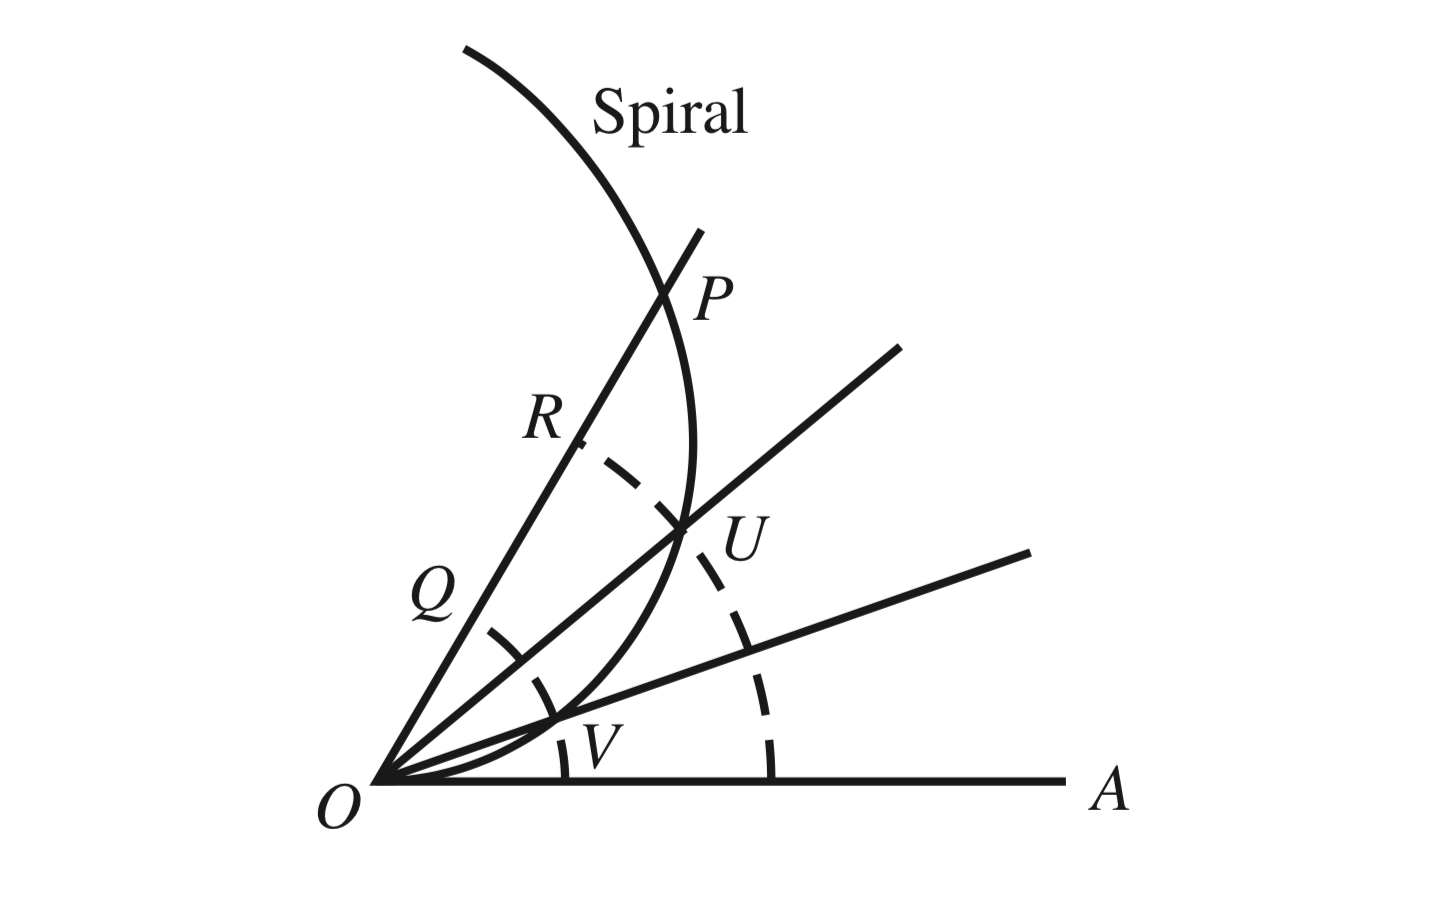
\includegraphics[width = .50\textwidth]{spiral.png}
    \end{center}  

    \solution Recall that the Archimedean spiral is defined by a parametric equation of the form, 
    \begin{equation*}
      r = a\theta
    \end{equation*}
    for some $a>0$. Note that by construction we have,
    \begin{equation*}
      OP = a(\angle AOP).
    \end{equation*}
    Solving for $a$ gives us, 
    \begin{equation*}
      a = \frac{OP}{\angle AOP}.
    \end{equation*}
    Solving for $\angle AOU$ in terms of $\angle AOP$ using the fact that by construction $OU = \frac{2}{3} OP$,
    \begin{align*}
      OU &= \frac{OP}{\angle AOP} (\angle AOU),\\
      \frac{2}{3}OP &= \frac{OP}{\angle AOP} (\angle AOU),\\
      \frac{2}{3} &= \frac{1}{\angle AOP} (\angle AOU),\\
      \frac{2}{3}{\angle AOP} &= \angle AOU.\\
    \end{align*}
    Similarly solving for for $\angle AOV$ in terms of $\angle AOP$ using the fact that by construction $OV = \frac{1}{3} OP$,
    \begin{align*}
      OV &= \frac{OP}{\angle AOP} (\angle AOV),\\
      \frac{1}{3}OP &= \frac{OP}{\angle AOP} (\angle AOV),\\
      \frac{1}{3} &= \frac{1}{\angle AOP} (\angle AOV),\\
      \frac{1}{3}{\angle AOP} &= \angle AOV.\\
    \end{align*}
Thus $\angle AOP$ is trisected by points $V$ and $U$.


\end{exercise}



\textbf{Reflection:}
\begin{enumerate}
  \item I had a really hard time doing sexagesimal division in problem 4b. At first I was solving for the circumference
   multiplying the 360 by the chord length and then dividing by 120. It was much easier to simplify the 360/120 to get 3
  and then multiply by the chord length. 
\item I don't know if we were supposed to do something special for problem 7 but I was able to find both sequences by just 
considering the first few primes.                                                                                                                                                                                                                                                                                                                    
\end{enumerate}





\end{document}